\documentclass[UTF8]{article}%z指定文档类型
\usepackage[UTF8]{ctex}%显示中文
\usepackage{graphicx}%引用图包
\usepackage{amsfonts,amsmath,amssymb,amstext}%数学相关宏包
\usepackage{color}

\begin{document}%文章开始


\title{计算机网络基础1}%文章题目
\maketitle% 显示上述标题信息

\section{网络分层概述与涉及名词解释}

\subsection{简图}

\begin{figure}[htb!]%插入图片
    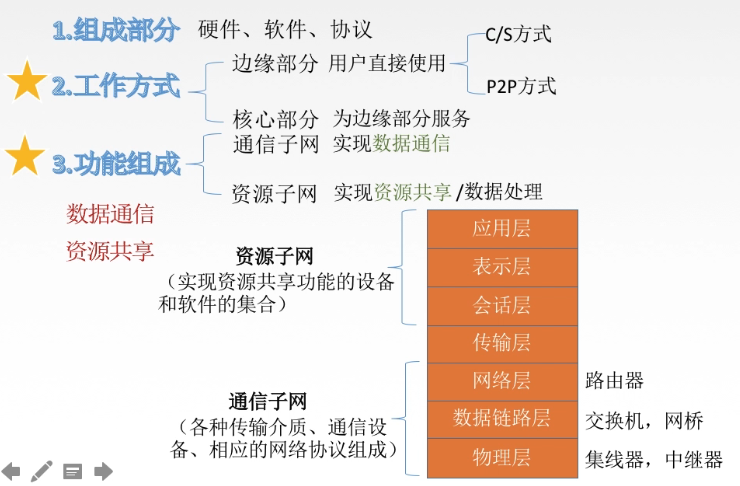
\includegraphics[width=1.0\textwidth]{1.1-1.png}
    \label{fig::1}
\end{figure}

\subsection{基本名词}

\begin{itemize}
    \item 分层:自下而上分别是物理层、数据链路层、网络层、传输层、会话层、表示层、应用层。越下面的层,越靠近硬件;越上面的层,越靠近用户;
    
    可以简化为物理层、数据链路层、网络层、传输层、应用层。

    \begin{figure}[htb!]%插入图片
        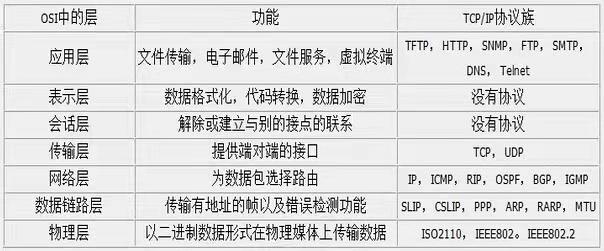
\includegraphics[width=1.0\textwidth]{1.1-2.jpg}
        \label{fig::2}
    \end{figure}

    \item 协议:每一层都是为了完成一种功能。为了实现这些功能,就需要大家都遵守共同的规则。则称都遵守的规则为"协议";
    \item 互联网协议:互联网的每一层,都定义了很多协议。这些协议的总称;
    \item MAC地址:(数据链路层)是一个用来确认网络设备位置的位址,唯一。本机(发送方)默认为FF-FF-FF-FF-FF-FF。
    \item IP地址:(网络层)类似于MAC地址,但IP地址是软件层面上的,可以随时修改,MAC 地址一般是无法修改的。在己方、对方IP未知的情况下,默认为0.0.0.0和255.255.255.255(DHCP服务器接受)。
    \item ARP协议:(网络层)地址解析协议(Address Resolution Protocol),根据IP地址获取物理地址的一个TCP/IP协议。
    \item MAC 地址表:存在于交换机中,用于映射 MAC 地址和它的\textcolor{red}{端口};通过以太网内各节点之间不断通过交换机通信,不断完善起来的;
    \item 路由表:存在于路由器中,用于映射 IP 地址(段)和它的\textcolor{red}{端口};是各种路由算法 + 人工配置逐步完善起来的;
    \item ARP 缓存表:存在于电脑和路由器中,用于缓存 IP 和 MAC 地址的映射关系;不断通过 ARP 协议的请求逐步完善起来的;
\end{itemize}

\subsection{基本设备}

\subsubsection{集线器hub}

\begin{itemize}
    \item 用处:对接收到的信号进行再生整形放大,以扩大网络的传输距离;
    \item 特点:发送数据时没有针对性;
    \item 处于物理层;
\end{itemize}

\subsubsection{交换机}

\begin{itemize}
    \item 用处:同集线器;
    \item 特点:只发给目标MAC地址指向的那台电脑;存有MAC地址表;
    \item 处于数据链路层;
\end{itemize}

\subsubsection{路由器}

\begin{itemize}
    \item 用处:作为一台独立的拥有 MAC 地址的设备,并且可以把数据包做一次转发;
    \item 特点:路由器的每一个端口,都有独立的 MAC 地址!

            其端口往往作为默认网关;

            存有路由表、ARP缓存表;

    \item 处于网络层;
\end{itemize}

\subsection{网络层下的数据传输过程}

已知发送方A的IP、MAC,接收方B的IP,进行信息传递:

\begin{itemize}
    \item A通过子网掩码计算A与B是否处于同一子网内:
    
    if(同一子网)  

        \qquad A通过ARP协议直接获得对方MAC码;

    else \quad A通过ARP获得默认网关MAC码;
        

        将源MAC地址与对方或网关的MAC地址封装在数据链路层头部;

        将源IP地址和目的IP地址封装在网络层头部;

        将数据传递给交换机; 

        (注意从始至终这个数据包的两个IP地址都是不变的,只有MAC地址在不断变化)

    \item 交换机数据发送:
    
    if(数据的MAC地址为网关MAC) 
        
    \qquad 将数据转发给网关即路由器的对应端口;
    
    else \quad 直接将数据转发给子网下的对方的对应端口
         
         \qquad or 全部端口(没找到MAC地址的情况);end;

    \item 路由器数据发送:
    
    通过路由表查找B的IP地址与端口的对应关系;

    if(没有找到)
    
    \qquad 返回一个路由不可达的数据包;end;

    else \quad 按照映射关系从指定端口发出去;

    数据到达指定端口对应的路由器;
    
    路由器通过ARP表获得B的IP地址对应的MAC码;

    (IP地址为同一路由器下则直接通过该路由器的ARP表获得MAC码)

    将其封装在数据链路层头部;

    通过路由器的路由表的映射关系获得B的IP地址对应的端口;
    
    将数据发送给对应的(交换机)端口;

    \item 交换机数据发送
    
    查询MAC地址表,确定B的对应端口,发送数据;end;

\end{itemize}

\subsection{物理层}

就是把电脑连接起来的物理手段。它主要规定了网络的一些电气特性。

\subsection{数据链路层}

它在"实体层"的上方,确定了0和1的分组方式(即确定了电信号的解读方式)。

具有以\textbf{太网协议}。

\subsubsection{以太网协议(Ethernet)}

\begin{itemize}
    \item 一组电信号构成一个数据包,叫做"帧"(\textcolor{red}{Frame})。每一帧分成两个部分:标头(Head)和数据(Data)。
    \item "标头"包含数据包的一些说明项,比如发送者、接受者、数据类型等等;"数据"则是数据包的具体内容。
    \item "标头"的长度,固定为22字节。"数据"的长度,最短为46字节,最长为1500字节。因此,整个"帧"最短为68字节,最长为1522字节。如果数据很长,就必须分割成多个帧进行发送。
    
    帧frame:|=head2=|==data2==|

\end{itemize}

广播:以太网采在传输数据包时用了一种很"原始"的方式,它不是把数据包准确送到接收方,而是向本网络内所有计算机发送,让每台计算机自己判断,是否为接收方。

\subsection{网络层}

它作用是引进一套新的地址,使得能够区分不同的计算机是否属于同一个子网络。这套地址就叫做"网络地址",简称"网址"。

网络地址用于确定计算机所在的子网络,MAC地址则将数据包送到该子网络中的目标网卡。

\subsubsection{ARP协议}

通过IP地址,得到同一个子网络内的主机MAC地址,可以把数据包发送到任意一台主机;或获得网关的MAC地址。

\subsubsection{IP协议}

\begin{itemize}
    \item 作用:一个是为每一台计算机分配IP地址,另一个是确定哪些地址在同一个子网络。
    \item 分类:IPV4为32字节,IPV6为128字节。
    
    以IPV4为例:8+8+8+8,即11111111.11111111.11111111.11111111,换算成十进制为255.255.255.255。

    地址分成两个部分,前一部分代表网络,后一部分代表主机。
    \item 处于同一个子网络的电脑,它们IP地址的网络部分必定是相同的。但网络部分长度不确定,通过子网掩码来确定。
    \item 子网掩码:表示子网络特征的一个参数,在形式上等同于IP地址,它的网络部分全部为1,主机部分全部为0。
    \item 判断方法:将两个IP地址与子网掩码分别进行AND运算(两个数位都为1,运算结果为1,否则为0),然后比较结果是否相同,如果是的话,就表明它们在同一个子网络中,否则就不是。
\end{itemize}

\textbf{IP数据包}

\begin{itemize}
    \item 根据IP协议发送的数据,就叫做IP数据包(\textcolor{red}{Packet})。
    \item IP地址也直接包含在以太网数据包的"数据"部分,因此完全不用修改以太网的规格。\textcolor{red}{上层的变动完全不涉及下层的结构}。
    \item IP数据包也分为"标头"和"数据"(payload)两个部分:"标头"部分主要包括版本、长度、IP地址等信息,"数据"部分则是IP数据包的具体内容。
    
    |=head2=|=head3=|==data3==|或|=head2=|=packet=|
    
    包packet:|=head3=|==data3==|

    \item "标头"部分的长度为20到60字节,整个数据包的总长度最大为65,535字节。因此,理论上,一个IP数据包的"数据"部分,最长为65,515字节。(大于之前的以太网数据包,可分割)
    
    \item 而以太网数据包的"数据"部分最长只有1500字节。因此,如果IP数据包超过了1500字节,它就需要分割成几个以太网数据包分开发送了。

\end{itemize}

\subsubsection{ICMP协议}

Internet Control Message Protocol,是IP的一部分,在IP协议栈中必须实现。ICMP的内容是放在IP数据包的数据部分里,并来互相交流的。

虽然从ICMP的报文格式来说,ICMP 是IP 的上层协议。但ICMP分担了IP的一部分功能。所以被认为是与IP同层的协议。

ICMP主要用于在主机与路由器之间传递控制信息,包括报告错误、交换受限控制和状态信息等。其在沟通之中,主要是透过不同的类别(Type)与代码(Code)让机器来识别不同的连线状况。

\textbf{用途:}

1. 网关或者目标机器利用ICMP与源通讯;

2. 当出现问题时,提供反馈信息用于报告错误;

\textbf{特点:}

1. 其控制能力并不用于保证传输的可靠性;

2. 它本身也不是可靠传输的;

3. 并不用来反映ICMP报文的传输情况。

\textbf{报文格式:}
\begin{itemize}
    \item ICMP报文包含在IP数据报中,属于IP的一个用户,IP头部就在ICMP报文的前面,所以一个ICMP报文包括IP头部、ICMP头部、ICMP报文。
    
    \begin{figure}[htb!]%插入图片
        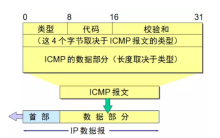
\includegraphics[width=0.6\textwidth]{1.7-1.png}
    \end{figure}

    \item IP首部字段包括:1)协议、2)源IP地址、3)目的IP地址、4)生存时间;
    \item ICMP数据部分字段包括:5)类型、6)代码、7)选项数据;
    \item IP头部的协议(Protocol)值为1就说明这是一个ICMP报文,ICMP头部中的类型(Type)域用于说明ICMP报文的作用及格式,此外还有一个代码(Code)域用于详细说明某种ICMP报文的类型,所有数据都在ICMP头部后面。
\end{itemize}

TYPE和Code部分可参考:

https://baike.baidu.com/item/ICMP/572452?fr=aladdin 

\textbf{应用:}

1. ping,利用 ICMP 协议包来侦测另一个主机是否可达。

2. Traceroute,用来侦测主机到目的主机之间所经路由情况。


\subsection{传输层}

它的作用是立"端口到端口"的通信(区别于"网络层"的功能是建立"主机到主机"的通信),实现主机的程序间的交流。

\subsubsection{端口(port)}

\begin{itemize}
    \item 用于表示数据包到底供哪个程序(进程)使用,它其实是每一个使用网卡的程序的编号。每个数据包都发到主机的特定端口,所以不同的程序就能取到自己所需要的数据。
    \item "端口"是0到65535之间的一个整数(正好16个二进制位)。0到1023的端口被系统占用,用户只能选用大于1023的端口,应用程序会随机选用一个端口,然后与服务器的相应端口联系。
\end{itemize}

必须在数据包中加入端口信息,这就需要新的协议。该层的数据包称为\textcolor{red}{Segment}。

\subsubsection{数据格式}

不论是UDP协议还是TCP协议,其格式都为“标头”+“数据”格式,如下所示,其中Segment为TCP协议下的传输包的基本单元,datagram为UDP协议下的传输包基本单元。

|=head2=|=head3=|=head4=|==data4==|
    
或|=head2=|=head3=|==Segment/datagram==|,

其中Segment/datagram:|=head4=|==data4==|

\subsubsection{UDP协议}

用户数据报协议(UDP,User Datagram Protocol)是面向数据报的、不可靠的、无序的传输协议。其为应用程序提供了一种无需建立连接就可以发送封装的 IP 数据包的方法。

特点:

\begin{itemize}
    \item 只需要知道对方的ip地址,将数据报一份一份的发送过去就可以了,其他的作为发送方,都不需要关心。
    \item 优点是比较简单,容易实现,不存在建立连接需要的时延;但是缺点是可靠性较差,一旦数据包发出,无法知道对方是否收到。
    \item 为了解决这个问题,提高网络可靠性,需要采用TCP协议。
\end{itemize}

\textbf{报文相关:}

\begin{itemize}
    \item 类似于IP数据包,UDP数据包也称为报文(datagram),整个报文也被放入IP数据包的"数据"部分。
    \item 报文(message):一般指完整的信息,传输层实现报文交付。将位于应用层的信息分组称为报文。
    \item 报文段(segment):是网络中交换与传输的数据单元,也是网络传输的单元。记为组成报文的每个分组。将运输层分组称为报文段。
\end{itemize}

数据表示:

\subsubsection{TCP协议(TCP)}

传输控制协议(TCP,Transmission Control Protocol)是一种面向连接的、可靠的、基于字节流的传输层通信协议。其作用是,保证数据通信的完整性和可靠性,防止丢包。

特点:

\begin{itemize}
    \item 可以近似认为,它就是有确认机制的UDP协议,每发出一个数据包都要求确认。
    \item TCP数据包没有长度限制,理论上可以无限长,但是为了保证网络的效率,通常TCP数据包的长度不会超过IP数据包的长度,以确保单个TCP数据包不必再分割。
    \item 数据包同样称为报文。
\end{itemize}

\subsection{应用层}

"应用层"的作用,就是规定应用程序的数据格式,从而对应用程序收到"传输层"的数据进行解读。

举例来说,TCP协议可以为各种各样的程序传递数据,比如Email、WWW、FTP等等。那么,必须有不同协议规定电子邮件、网页、FTP数据的格式,这些应用程序协议就构成了"应用层"。这是最高的一层,直接面对用户。它的数据就放在TCP数据包的"数据"部分。

包括DHCP协议、TFTP协议、HTTP协议、SNMP协议、FTP协议、SMTP协议、DNS协议、telnet协议。

通过以上五层处理,以太网数据包最终为如下格式:

\begin{figure}[htb!]%插入图片
    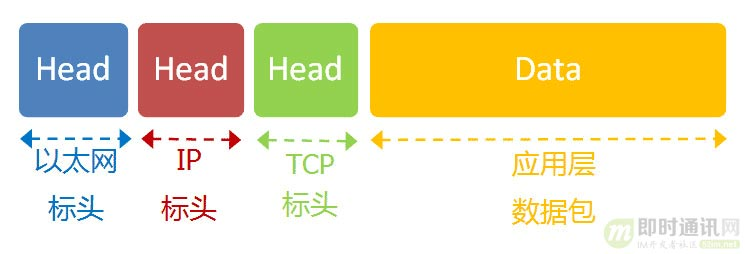
\includegraphics[width=1.0\textwidth]{1.9-1}
    \label{fig::3}
\end{figure} 

\subsubsection{DHCP协议}

静态IP地址:计算机在连接互联网时,需要知道本机的IP地址、子网掩码、网关的IP地址、DNS的IP地址。由于它们是给定的,计算机每次开机,都会分到同样的IP地址。

动态IP地址:指计算机开机后,会自动分配到一个IP地址,不用人为设定。它使用的协议叫做DHCP协议。

协议简介:

\begin{itemize}
    \item 这个协议规定,每一个子网络中,有一台计算机负责管理本网络的所有IP地址,它叫做"DHCP服务器"。新的计算机加入网络,必须向"DHCP服务器"发送一个"DHCP请求"数据包,申请IP地址和相关的网络参数。
    \item \textcolor{red}{它是一种应用层协议,建立在UDP协议之上}。即DHCP数据包在UDP数据包的“数据”部分。
    \item 初次数据传递流程:数据打包完成后,以太网广播发送,同一个子网络的每台计算机都收到了这个包。因为接收方的MAC地址是默认地址(FF-FF-FF-FF-FF-FF),看不出是发给谁的,所以每台收到这个包的计算机,还必须分析这个包的IP地址。当看到发出方IP地址是0.0.0.0,接收方是255.255.255.255,于是DHCP服务器知道"这个包是发给我的",而其他计算机就可以丢弃这个包。
    \item 处于应用层。
\end{itemize}

\subsubsection{TFTP协议}

简单文件传输协议(TFTP,Trival File Transfer Protocal)该协议在熟知端口69上使用UDP服务。常用于无盘工作站或路由器从别的主机上获取引导配置文件,由于TFTP报文比较小,能够迅速复制这些文件。

特点:

1. 所占用的内存小;

2. 支持ASCII码或二进制传送;

3. 由于TFTP是设计用于系统引导进程,其分组不提供用户名和口令。

4. 服务端向用户端发送数据大小固定为512B,不足则认为其是最后报文。如果最后一个数据报的长度正好为512B,此时服务器进程会再次发送一个包含0字节数据的DATA报文。

5. 在TFTP的ACK报文中,ACK中的块号表示的是本次成功收到的数据块,而不是下一个期望的下一个数据块。每一个512B的块大小为1。

传输过程描述:(FTP客户向TFTP服务器发送读请求为例)

\begin{itemize}
    \item 服务器使用熟知端口号69被动打开连接;
    \item 客户主动打开连接,它使用\textbf{临时端口}作为源端口而以熟知端口69作为目的端口,向服务器进程发送RRQ报文;
    \item 服务器主动打开连接,它使用新的临时端口作为源端口,而使用收到的来自客户的临时端口作为目的端口,向TFTP客户进程发送DATA报文(2B操作码,2B数据块的块号K,512B数据);
    \item 客户收到服务器的报文后,发送4B的ACK(2B的操作码和2B的数据块号)给TFTP服务器,告诉它之前发送给客户的数据报已经收到;
    \item 重复步骤3-4,直到所有请求的数据发送完毕。
\end{itemize}

五种报文:

\begin{itemize}
    \item RRQ:操作码=1,读请求,服务器返回一个块编号为1的DATA报文。
    \item WRQ:操作码=2,写请求,服务器返回的是块编号为0的ACK报文。
    \item DATA:操作码=3,由客户或服务器使用(\textbf{写者发送}),用于传送数据块。所有的块都用数字顺序编码,从1开始。
    \item ACK:操作码=4,块号表示向对方确认它所收到的块号,WRQ情况下服务器返回的是一个块号为0的ACK报文,表示服务器已经准备好了接收来自客户的数据报。
    \item ERROR:操作码=5,既可以由客户发送,也可以由服务器发送,当一条连接(如读连接或写连接)不能建立、或在数据传输中出现问题时使用。差错码定义了差错的类型,差错信息是一个可变字节,包含原文中的差错数据。
\end{itemize}

注意:TFTP报文没有差错检验和字段,所以接收端检验数据是否出现差错的唯一方法是通过分组该TFTP数据报的UDP首部中的检验和字段。

\subsubsection{HTTP协议}

超文本传输协议(HTTP,Hyper Text Transfer Protocol),用于从万维网(WWW:World Wide Web )服务器传输超文本到本地浏览器的传送协议。

HTTP协议工作于客户端-服务端架构为上。浏览器作为HTTP客户端通过URL向HTTP服务端即WEB服务器发送所有请求。Web服务器根据接收到的请求后,向客户端发送响应信息。

主要特点

\begin{itemize}
    \item 简单快速:客户向服务器请求服务时,只需传送请求方法和路径。请求方法常用的有GET、HEAD、POST。每种方法规定了客户与服务器联系的类型不同。由于HTTP协议简单,使得HTTP服务器的程序规模小,因而通信速度很快。
    \item 灵活:HTTP允许传输任意类型的数据对象。正在传输的类型由Content-Type加以标记。
    \item 无连接:无连接的含义是限制每次连接只处理一个请求。服务器处理完客户的请求,并收到客户的应答后,即断开连接。采用这种方式可以节省传输时间。
    \item 无状态:HTTP协议是无状态协议。无状态是指协议对于事务处理没有记忆能力。缺少状态意味着如果后续处理需要前面的信息,则它必须重传,这样可能导致每次连接传送的数据量增大。另一方面,在服务器不需要先前信息时它的应答就较快。
    \item 支持B/S及C/S模式。
\end{itemize}

\paragraph{URL}~{}

HTTP使用统一资源标识符(Uniform Resource Identifiers, URI)来传输数据和建立连接。URL(uniform resource locator,统一资源定位器)是一种特殊类型的URI,包含了用于查找某个资源的足够的信息。

以http://www.ass.com:8080/news/index.asp?boardID=5

\&ID=24618\&page=1\#name 为例,包括:

\begin{itemize}
    \item 协议部分:从头开始,以“//”为分隔符。意义为这网页所使用的协议。在Internet中可以使用多种协议,如HTTP,FTP等等。
    \item 域名部分:跟在“//”后面,到“:”为止。一个URL中,也可以使用IP地址作为域名使用;
    \item 端口部分:跟在域名后面的是端口,域名和端口之间使用“:”作为分隔符。非必须,无则采用默认端口。
    \item 虚拟目录部分:从域名后的第一个“/”开始到最后一个“/”为止。非必须。
    \item 文件名部分:从域名后的最后一个“/”开始到“?”为止;如果没有“?”,则到“\#”为止;如果都没有,那么到结束都是。非必须,如省略则使用默认的文件名。
    \item 锚部分:从“\#”开始到最后,都是锚部分。非必须。
    \item 参数部分:从“?”开始到“\#”为止之间的部分为参数部分,又称搜索部分、查询部分。参数可以允许有多个参数,参数与参数之间用“\&”作为分隔符。
\end{itemize}

注意:URI是以一种抽象的,高层次概念定义统一资源标识,而URL和URN(uniform resource name,统一资源命名)则是具体的资源标识的方式。URL和URN都是一种URI。

关于格式、可参考链接:

https://www.cnblogs.com/ranyonsue/p/5984001.html

http://www.52im.net/thread-1677-1-1.html

\subsubsection{SNMP协议}

是专门设计用于在 IP 网络管理网络节点(服务器、工作站、路由器、交换机及HUBS等)的一种标准协议。 SNMP使网络管理员能够管理网络效能,发现并解决网络问题以及规划网络增长。通过 SNMP 接收随机消息(及事件报告)网络管理系统获知网络出现问题。

\subsubsection{FTP协议}

文件传输协议(FTP,File Transfer Protocol)作为网络共享文件的传输协议,在网络应用软件中具有广泛的应用。FTP的目标是提高文件的共享性和可靠高效地传送数据。

在传输文件时,FTP 客户端程序先与服务器建立连接,然后向服务器发送命令。服务器收到命令后给予响应,并执行命令。FTP 协议与操作系统无关,任何操作系统上的程序只要符合 FTP 协议,就可以相互传输数据。

具体可参考:

https://blog.csdn.net/zhubao124/article/details/81662775

\subsubsection{SMTP协议}

简单邮件传输协议(SMTP,Simple Mail Transfer Protocol)是一组用于由源地址到目的地址传送邮件的规则,由它来控制信件的中转方式。SMTP协议属于TCP/IP协议簇,它帮助每台计算机在发送或中转信件时找到下一个目的地。

建立一个运行在接收端邮件服务器主机上的SMTP服务器端口号25之间的TCP连接。

\subsubsection{DNS协议}

\begin{itemize}
    \item DNS是一种可以将域名和IP地址相互映射的以层次结构分布的数据库系统。
    \item 作用:用来将域名转换为IP地址,从而在知道域名的情况下进行数据传输(也可以将IP地址转换为相应的域名地址)。
    \item 注意:域名和IP地址是多对一的关系。
\end{itemize}




 

\section{部分协议详解}

\subsection{协议关系简述}

最底层的以太网协议(Ethernet)规定了电子信号如何组成数据包(packet),解决了子网内部的点对点通信。但是,以太网协议不能解决多个局域网如何互通,这由 IP 协议解决。

IP 协议定义了一套自己的地址规则,称为 IP 地址。它实现了路由功能,允许某个局域网的 A 主机,向另一个局域网的 B 主机发送消息。

IP 协议只是一个地址协议,并不保证数据包的完整。如果路由器丢包(比如缓存满了,新进来的数据包就会丢失),就需要发现丢了哪一个包,以及如何重新发送这个包。这就要依靠 TCP 协议。

\subsection{IP协议}

\subsubsection{IP地址结构}

网络地址:网络地址位于IP地址的前段,可用来识别设备所在的网络。当组织或企业申请IP地址时,所获得的并非IP地址,而是取得一个唯一的、能够识别的网络地址。同一网络上的所有设备,都有相同的网络地址。IP路由的功能是根据IP地址中的网络地址,决定要将IP信息包送至所指明的那个网络。

主机地址:位于IP地址的后段,可用来识别网络上设备。同一网络上的设备都会有相同的网络地址,而各设备之间则是以主机地址来区别。

\subsubsection{五种地址等级}

5种等级分别使用不同长度的网络地址,因此适用于大、中,小型网络:

\begin{itemize}
    \item A类IP地址:由1个字节的网络地址和3字节主机地址组成,网络标识长度为8位,主机标识长度为24位。由于网络地址的最高位必须为“0”,且需要去除掉特殊的网段地址和广播地址,因此网络有126个($2^7-2=126$)。
    \item B类IP地址:由2个字节的网络地址和2字节主机地址组成。由于网络地址的最高位必须为“10”,且同样需要去除两特殊地址,因此网络有16,384个($2^{14}-2$)。
    \item C类IP地址:由3个字节的网络地址和1字节主机地址组成的,网络地址的最高位必须为“110”。同上。
    \item D类IP地址:第一个字节以1110开始,地址范围为:224.0.0.1到239.255.255.254。它是一个专门保留的地址,并不指向特定的网络,目前这一类地址被用在多点广播(Multicast)中。多点广播地址用来一次寻址一组计算机,它标识共享同一协议的一组计算机。
    \item E类IP地址:仅作实验和将来开发而保留,它以1111开始,全0(0.0.0.0)的IP地址指任意网络,全1的IP地址(255.255.255.255)是当前子网的广播。
\end{itemize}

\subsubsection{特殊IP地址}

\begin{itemize}
    \item 广播地扯:所有主机号部分为1的地址。分为直接广播地址和有限广播地址。

    在一特定子网中,主机地址部分为全I的地址称为直接广播地址。可以向任何指定的网络直接广播它的数据报。

    IP地址全为l的IP地址被称为有限广播地址或本地网广播地址,该地址被用作在本网络内部广播。

    \item 组播地址:即D类IP地址。实际上代表一组特定的主机。组播地址和广播地址的区别在于广播地址是按主机的物理位置来划分各组的(属于同一个子网),而组播地址指定一个逻辑组,参与该组的计算机可能遍布整个Internet。组播地址主要用于电视会议、视频点播等应用。
    \item 0地址:0.0.0.0代表本主机地址,网络上任何主机都可以用它来表示自己。主机号为0的IP地址从来不分配给任何一个单个的主机号为0。
    \item 回送地址:原本属于A类地址范围内的IP地址127.0.0.0~127.255.255.255却并没有包含在A类地址之内。任何一个以数字127开头的IP地址(127.x.x.x)都叫做回送地址(A类中以1开头的)。
    
    在每个主机上对应于IP地址127.0.0.1有个接口,称为回送接口。IP协议规定,当任何程序用回送地址作为目的地址时,计算机上的协议软件不会把该数据报向网络上发送,而是把数据直接返回给本主机。因此网络号等于127的数据报文不能出现于任何网络上,主机和路由器不能为该地址广播任何寻径信息。回送地址的用途是,可以实现对本机网络协议的测试或实现本地进程间的通信。
\end{itemize}

\subsection{TCP协议}

由之前可知,以太网数据包(packet)的大小是固定的1522字节。其中, 1500 字节是负载(payload),22字节是头信息(head)。而IP数据包在以太网数据包的负载里面,它的头信息最少需要20字节,所以 IP 数据包的负载最多为1480字节;TCP 数据包在 IP 数据包的负载里面,它的头信息最少需要20字节,因此TCP数据包的最大负载是1460字节。由于 IP 和 TCP 协议往往有额外的头信息,所以 TCP 负载实际为1400字节左右。

\subsubsection{TCP 数据格式}

\begin{figure}[htb!]%插入图片
    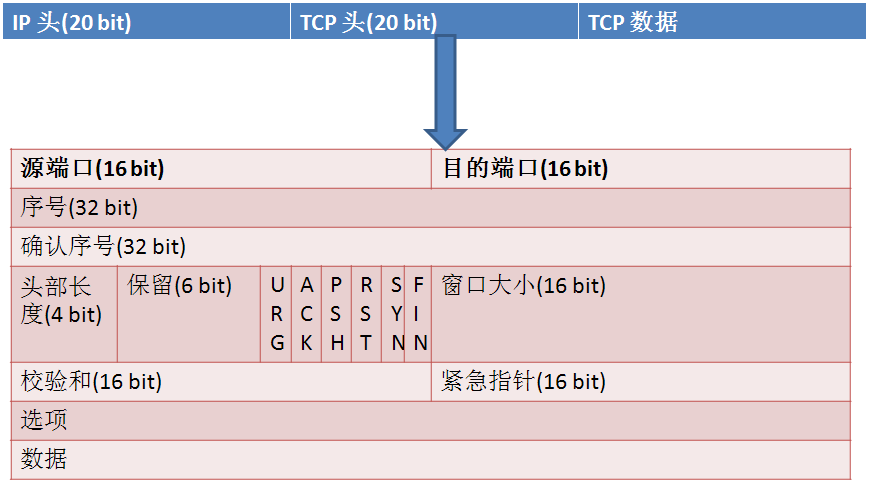
\includegraphics[width=0.9\textwidth]{2.3-1.png}
    \label{fig::5}
\end{figure}

\paragraph{a. 基本数据格式}~{}

\begin{itemize}
    \item 源端口和目的端口(Source Port And Destination Port):2字节,分别写入源端口号与目的端口号。
    \item 序列号(Sequence Number):4字节,用于发送的TCP数据包的编号。
    \item 确认序号(Acknowledgement Number):4字节,即Ack,示期望收到对方下一个报文段的第一个数据字节的序号。
    \item 头部长度(Offset):4位,即指数据偏移,指出 TCP 报文段的数据起始处距离 TCP 报文段的起始处有多远。这个字段实际上是指出 TCP 报文段的首部长度。(在此长度之后为报文段的数据)
    \item 保留(Reserved):6位,保留为今后使用,目前应置为 0。
    \item 标志位(TCP Flags):数据包的属性,用于控制 TCP 的状态机。
    \item 窗口(Window):2字节,指的是本机接收缓冲区的空闲空间(而不是发送窗口)。用于告诉对方:从本报文段首部中的确认号算起,接受方目前允许对方发送的数据量(以字节为单位)。
    \item 校验和(Checksum):2字节,校验和字段检验的范围包括首部和数据两部分。
    \item 紧急指针(Urgent Pointer):2字节,仅在 URG = 1时才有意义,它表示紧急数据相对序列号(Seq)的偏移。因此,紧急指针指出了紧急数据的末尾在报文段中的位置。
    \item 选项(TCP Options):长度可变,最长可达 40 字节。当没有使用“选项时”,TCP 的首部长度是 20 字节。
    \item 剩下为数据部分。
\end{itemize}

\paragraph{b. 标志位的FLAGS字段各位意义}~{}

\begin{itemize}
    \item 100000:URG(URGent)紧急位。为1时告诉系统此报文段中有紧急数据,应尽快传送,而不要按原来的排队顺序来传送,发送方的TCP就把紧急数据放到本报文段数据的最前面。
    
    URG标志位要与首部中的紧急指针字段配合使用,紧急指针指向数据段中的某个字节,(数据从第一个字节到指针所指的字节就是紧急数据)。
    
    注意即使窗口为0时也可以发送紧急数据,紧急数据不进入接收缓冲区直接交给上层进程,而不是等待缓冲区满后再交付。

    \item 010000:ACK(Acknowledgment)确认字符。为1时表示前面的确认号字段有效。TCP规定,连接建立后,ACK必须为1。
    \item 001000:PSH(push)推送。为1时表示对方收到该报文段后应当立即把数据提交给上层,而不是缓存起来。
    \item 000100:RST(rest)。为1时表明与主机的连接出现了严重错误(如主机崩溃),必须释放连接,然后再重新建立连接。或者说明上次发送给主机的数据有问题,主机拒绝响应。
    \item 000010:SYN(Synchronize Sequence Numbers)同步序列编号。为1时表示这是一个请求建立连接或同意建立连接的报文。当SYN=1,ACK=0时,表示这是一个请求建立连接的报文段;当SYN=1,ACK=1时,表示对方同意建立连接。
    \item 000001:FIN(标记数据是否发送完毕。)。标记数据是否发送完毕。为1时表示发送此报文段的发送方已经发送完了所有数据,以后不会也不能再发送数据,当另外一方也发送FIN时,则连接断开。
\end{itemize}

注意:ACK是连接建立的标志,为0或1;而Ack则是确认序号,其值为Seq+1。Seq除第一次随机产生、其余均是接着自己传输序号的。

\paragraph{c. TCP 数据包的序列号(Seq)}~{}

较大的数据往往拆分为若干个包发送,在发送的时候,TCP 协议为每个包编号(sequence number,简称 Seq),以便接收的一方按照顺序还原。

第一个包的编号是一个随机数。若把第一个包称为1号包。假定这个包的负载长度是100字节,那么可以推算出下一个包的编号应该是101。每个数据包都可以得到两个编号:自身的编号,以及下一个包的编号,接收方由此知道,应该按照什么顺序将它们还原成原始文件。(即编号可知包的负载(payload))

\paragraph{d. TCP 数据包的组装}~{}

\begin{itemize}
    \item 应用程序需要的数据放在 TCP 数据包里面,有自己的格式(比如 HTTP 协议)。
    \item 由操作系统来组装TCP数据包,然后由应用程序来处理包里的数据。
    \item TCP 数据包里面有一个端口(port)参数,用来指定转交给监听该端口的应用程序。
    \item TCP 没有提供任何机制来表示\textbf{原始文件}的大小,这由应用层的协议来规定。
    \item 应用程序收到组装好的原始数据,以浏览器为例,就会根据 HTTP 协议的 Content-Length 字段正确读出一段段的数据。这也意味着,一次 TCP 通信可以包括多个 HTTP 通信。
\end{itemize}

\subsubsection{连接管理}

基本原理:(TCP是面向连接的,UDP不是面向连接的)。TCP通过连接这个动作让接收方知道发送方想要发送数据给它,如果接收方允许,则连接建立,这时双方之间便可以进行数据传输,接收到数据之后须确认数据收到。

(认为主动发送方为客户端,被动接受方为服务端)

\paragraph{a. 连接的建立——三次握手}~{}

\begin{itemize}
    \item 客户端首先向服务端发出建立连接的请求$^1$并等待服务端的确认。
    
    ==>SYN=1,ACK=0,seq=x$^2$,Ack=NULL

    \item 服务端收到建立连接的请求之后,如果同意建立连接,则向客户端发送确认,并等待客户端确认该TCP报文已经收到。
    
    <==SYN=1,ACK=1,seq=y,Ack=x+1

    \item 客户端收到服务端的确认报文段之后,再次向服务端发送确认,确认服务器的确认报文已经收到。
    
    ==>SYN=0,ACK=1,seq=x+a$^3$,Ack=y+1

\end{itemize}

注意:

1. 上述信息均为TCP报文段。

2. x、y均为随机产生的值,表示连接初始时发送的数据包编号,对方确认后返回的Ack值在此基础上加1。

3. a表示第三次握手发送的数据包大小,注意不是x+1+a,因为返回的+1是表示需求从这个序号开始的包。

\paragraph{b. 连接的断开——四次握手}~{}

四次原因:通过TCP三次握手建立的通信属于全双工通信,因此每个方向都必须单独地进行关闭。

\begin{itemize}
    \item 客户端发送一个主动关闭连接请求,用来关闭客户到服务端的数据传送。

        ==>FIN=1,ACK=1,seq=m,Ack=k$^1$

    \item 服务端收到这个FIN,它发回一个ACK,确认序号为收到的序号加1。和SYN一样,一个FIN将占用一个序号。

        <==FIN=0,ACK=1,seq=n,Ack=m+1

    \item 服务端关闭客户端的连接,发送一个FIN给客户端。
    
        <==FIN=1,ACK=1,seq=w$^2$,Ack=m+1$^3$

    \item 客户端发回ACK报文确认,并将确认序号设置为收到序号加1。
    
        ==>FIN=0,ACK=1,seq=m$^4$,Ack=w+1

    \item 特殊1:如果两边同时同时发起主动关闭,则两边互相确认后直接关闭。
    
        ==>FIN=1,ACK=1,seq=m,Ack=j+1\& FIN=1,ACK=1,seq=n,Ack=k+1

        <==ACK=1,Ack=m+1,seq=j \& ACK=1,Ack=n+1,seq=k;

    \item 特殊2:服务端收到FIN后也可直接回复ACK和FIN。
    
        <==FIN=1,ACK=1,seq=n,Ack=m+1
        
\end{itemize}

注意:

1. k=n-b+1,表示服务端传输的数据包累计数目+1,m表示客户端传输的累计数目。

2. w=n+a,其中a为第三次握手即最后一次服务端->主机数据传输中数据包数量(Ack+1而seq不用)。

3. 由于两次服务端->客户端传输过程中没有客户端到服务端的数据,因此两次Ack一样。

4. 由于无客户端到服务端的数据,因此两次seq一样。



\paragraph{c. TCP传输连接有限状态机}~{}

把在TCP传输连接的建立和释放中的通信双方主机的这些状态称之为“有限状态机”(Finite State Machine,FSM):

\begin{itemize}
    \item $CLOSED$:表示当前主机没有活动的传输连接或没有正在进行传输连接。
    \item $LISTEN$:表示服务器端的某个SOCKET处于监听状态,可以接受连接了。正常情况下主机开机后就一直处于该状态。
    \item $SYN\_SENT$:(客户端状态)当客户端SOCKET执行CONNECT连接时,其发送SYN=1、ACK=0报文后所进入的状态。持续到服务端发送确认报文ACK=1。
    \item $SYN\_RCVD$:(服务端状态)表示服务端在收到一个连接请求并回复SYN=1,ACk=1的确认后所进入的状态。一般很短暂,持续到收到客户端的SYN=0、ACK=1的确认后。
    \item $ESTABLISHED$:通信双方处于正常数据传输状态。
    \item $FIN\_WAIT\_1$:(客户端状态)表示客户端调用close,主动发送关闭连接的FIN=1请求,等待对方确认的状态。一般很短暂,持续到服务端发送确认报文ACK=1。
    \item $CLOSE\_WAIT$:(服务端状态)服务端收到客户端的主动关闭连接请求,并已回复确认报文ACK=1后所进入的状态。持续到服务端数据传递完毕,发送关闭传输连接请求FIN=1。
    \item $FIN\_WAIT\_2$:(客户端状态)客户端已经收到对方对主动关闭连接请求的确认ACK=1后的状态$^1$。持续到对方发送关闭传输连接请求FIN=1。$^2$
    \item $TIME\_WAIT$:(客户端状态)在客户端接收到对方关闭传输连接请求FIN=1并回复确认ACK=1后所进入的状态。持续$2MSL^3$时间,然后回到$CLOSED$可用状态。
    \item $LAST\_ACK$:(服务端状态)服务端发送完关闭传输连接请求FIN=1之后的状态。持续到收到客户端回复确认ACK=1。
    \item $CLOSING$:如果双方几乎在同时close一个SOCKET的话,那么就出现了双方同时发送FIN报文的情况,也就会出现CLOSING状态,表示双方都正在关闭SOCKET连接。这种状态比较特殊,实际情况中很少见,属于一种比较罕见的例外状态。
\end{itemize}

注意:

1.这是在关闭连接时,客户端和服务器两次握手之后的状态。是著名的半关闭的状态,在这个状态下,应用程序还有接受数据的能力,但是已经无法发送数据。但是也有一种可能是,客户端一直处于FIN-WAIT-2状态,而服务器则一直处于$CLOSE\_WAIT$状态,而直到应用层来决定关闭这个状态;

2.如果在$FIN\_WAIT\_1$状态下,收到了对方同时含有FIN=1和ACK=1的报文时,可以直接进入$TIME\_WAIT$状态。

3.MSL:(Maximum Segment Lifetime)报文最大生存时间。

注意:TTL:“生存时间”,由源主机设置的初始值,不是存的具体时间,而是存储了一个ip数据报可以经过的最大路由数,每经过一个处理它的路由器此值就减1,当此值为0则数据报将被丢弃,同时发送ICMP报文通知源主机。MSL要大于等于TTL。

\paragraph{d. TCP传输连接图解}~{}

三次握手:

\begin{figure}[htb!]%插入图片
    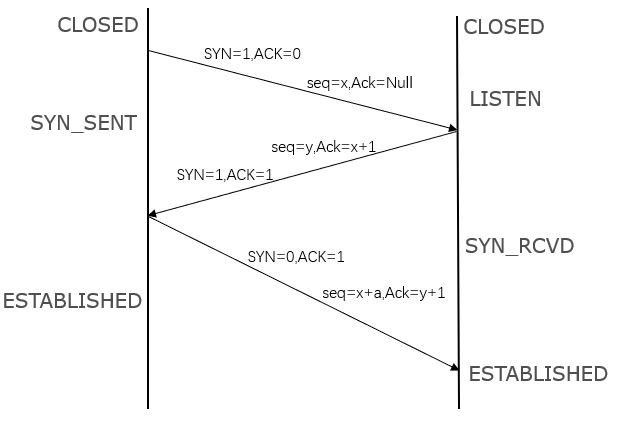
\includegraphics[width=0.6\textwidth]{2.3-2.png}
    \label{fig::6}
\end{figure}

四次握手:

\begin{figure}[htb!]%插入图片
    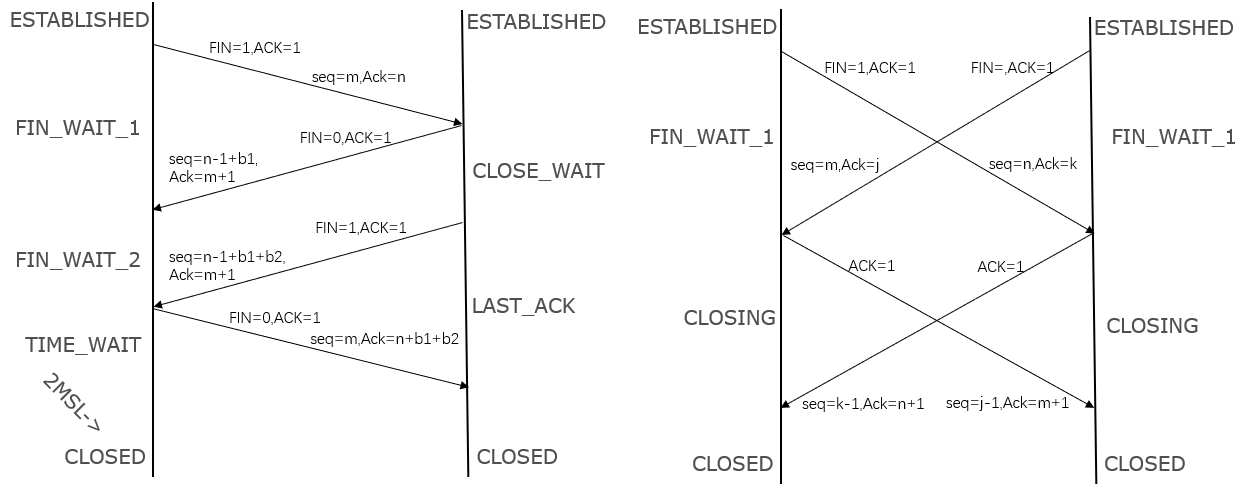
\includegraphics[width=1.1\textwidth]{2.3-3.png}
    \label{fig::7}
\end{figure}

\subsubsection{TCP流量控制(滑动窗口协议)}

TCP流量控制主要是针对接收端的处理速度不如发送端发送速度快的问题,消除发送方使接收方缓存溢出的可能性。同时发送方也不必每发一个分组就停下来等待确认。因此可以加速数据的传输,提高网络吞吐量。

TCP流量控制主要使用滑动窗口协议:

\begin{itemize}
    \item 滑动窗口是接受数据端使用的窗口大小,用来告诉发送端接收端的缓存大小,以此可以控制发送端发送数据的大小,从而达到流量控制的目的。
    \item 发送方在发送过程中始终保持着一个发送窗口,表示可以接受的数据包的数目,只有落在发送窗口内的包才允许被发送。
    \item 接收方也维持着一个接收窗口,只有落在接收窗口内的包才允许接收。
    
    接受方返回的ACK包中就会包含此窗口信息win=n。

\end{itemize}

注意:

1. 发送数据包大小不一定为窗口大小;

2. 发送窗口在收到确认后右边沿会右移,否则不动,但不会左移。

\subsubsection{TCP拥塞控制}

流量控制是通过接收方来控制流量的一种方式;而拥塞控制则是通过发送方来控制流量的一种方式。

用于解决TCP发送方可能因为IP网络的拥塞而被遏制的问题。

TCP拥塞控制的几种方法:慢启动,拥塞避免,快重传和快恢复。

\paragraph{0.拥塞窗口(cwnd)}~{}

发送方维持的一个状态变量,其大小取决于网络的拥塞程度,并且动态变化。

发送方发送的窗口实际大小=min(cwnd,接受端接收窗口大小)。

原则:只要网络没有出现拥塞,拥塞窗口就增大一些,以便把更多的分组发送出去。但只要网络出现拥塞,拥塞窗口就减小一些,以减少注入到网络中的分组数。

\paragraph{a. 慢启动(slow start)}~{}

\begin{itemize}
    \item 是传输控制协议使用的一种阻塞控制机制。开始的时候,发送得较慢,然后根据丢包的情况,调整速率:如果不丢包,就加快发送速度;如果丢包,就通过拥塞控制的其他方法来降低发送速度。
    \item 拥塞窗口的初始值为1,每收到一个对发出的\textcolor{red}{数据段}的ACK确认,便将拥塞窗口的值增加1(每完成一次传输轮次,拥塞窗口的值就翻倍,即拥塞窗口随着传输轮次的增加成指数增长)。
    \item 存在阈值:慢启动门限(ssthresh)(初始值为16),与慢启动关系如下:
    
    当 拥塞窗口 < 阈值 时,使用慢启动算法;

    当 拥塞窗口 > 阈值 时,使用拥塞避免算法;

    当 拥塞窗口 = 阈值时,既可以使用慢启动算法,也可时使用拥塞避免算法。
\end{itemize}

\paragraph{b. 拥塞避免}~{}

原理:cwnd的值不再指数级往上升,开始加法增加。此时当窗口中所有的报文段都被确认时,cwnd的大小再加1,从而慢慢增加调整到网络的最佳值。(即到阈值后cwnd不再是指数增长,而是+1增长)

注意:不能完全能够避免拥塞。

\textbf{加速递减机制:}

发送端发送数据时,出现了定时器超时timeout,便执行该机制:

1. 立刻将慢启动门限置为当前拥塞窗口大小的一半;

2. 拥塞窗口的值重置为1;

3. 再执行慢启动机制。

\paragraph{d. 快速重传}~{}

要求接收方每收到一个失序的TCP报文段后就立即发出重复确认(为了使发送方及早知道没有到达对方)而不要等待自己发送数据时才进行确认:

发送方只要连续收到3个同一个包的确认就应当立即重传未被确认的报文段,而不用等timeout。

\paragraph{e. 快恢复}~{}

当发送端收到连续三个重复的确认时,发送端认为网络很可能没有发生拥塞,因此执行“乘法减小”算法,而非“加速递减”机制。

\textbf{“加速递减”机制:}

1. 把慢启动门限置为当前拥塞窗口大小的一半;

2. 拥塞窗口不设置为1,而是设置为慢启动门限减半后的数值;

3. 这之后采用慢启动机制。

\subsection{UDP协议}

\paragraph{数据包格式:}~{}

\begin{itemize}
    
    \item 数据包由"标头"、"数据"两部分组成,格式几乎就是在数据前面,加上端口号。
    \item "标头"部分主要定义了发出端口和接收端口,"数据"部分就是具体的内容。
    \item UDP数据包"标头"部分一共只有8个字节,总长度不超过65,535字节,正好放进一个IP数据包。8字节由4个字段构成,每个字段都是两个字节,字段:
    
    1.源端口: 源端口号,需要对方回信时选用,不需要时全部置0;

    2.目的端口:目的端口号,在终点交付报文的时候需要用到;

    3.长度:UDP的数据报的长度(包括首部和数据)其最小值为8(只有首部情况);

    4.校验和:检测UDP数据报在传输中是否有错,有错则丢弃;(该字段是可选的,当源主机不想计算校验和,则直接令该字段全为0)
\end{itemize}

\paragraph{每次 UDP 发送的数据报大小:}~{}

影响因素:

1. UDP协议本身,UDP协议中有16位的UDP报文长度,那么UDP报文长度不能超过$2^16=65536$;

2. 以太网数据帧的长度,数据链路层的MTU(最大传输单元);

3. socket的UDP发送缓存区大小。

结论:

在Internet下MTU的值为576字节,所以在internet下使用UDP协议,每个数据报最大的字节数为: 576-20-8=548。

(注意正如之前所述:IP协议本身封装后包头占20~60个字节)

\paragraph{UDP丢包可能原因:}~{}

\begin{itemize}
    \item 数据报分片重组丢失,UDP本身有CRC检测机制,会抛弃掉丢失的UDP包;
    \item UDP 缓冲区填满:当接收方UDP缓冲区被填满的时候,这个时候再过来的数据报就都被丢弃了。
\end{itemize}

\paragraph{UDP校验简介:}

在计算校验和的时候,需要在UDP数据报之前增加12字节的伪首部,伪首部并不是UDP真正的首部。只是在计算校验和,临时添加在UDP数据报的前面,得到一个临时的UDP数据报。校验和就是按照这个临时的UDP数据报计算的。伪首部既不向下传送也不向上递交,而仅仅是为了计算校验和。这样的校验和,既检查了UDP数据报,又对IP数据报的源IP地址和目的IP地址进行了检验。

UDP校验和的计算方法和IP数据报首部校验和的计算方法相似,都使用二进制反码运算求和再取反,但不同的是:IP数据报的校验和之检验IP数据报和首部,但UDP的校验和是把首部和数据部分一起校验。

\begin{figure}[htb!]%插入图片
    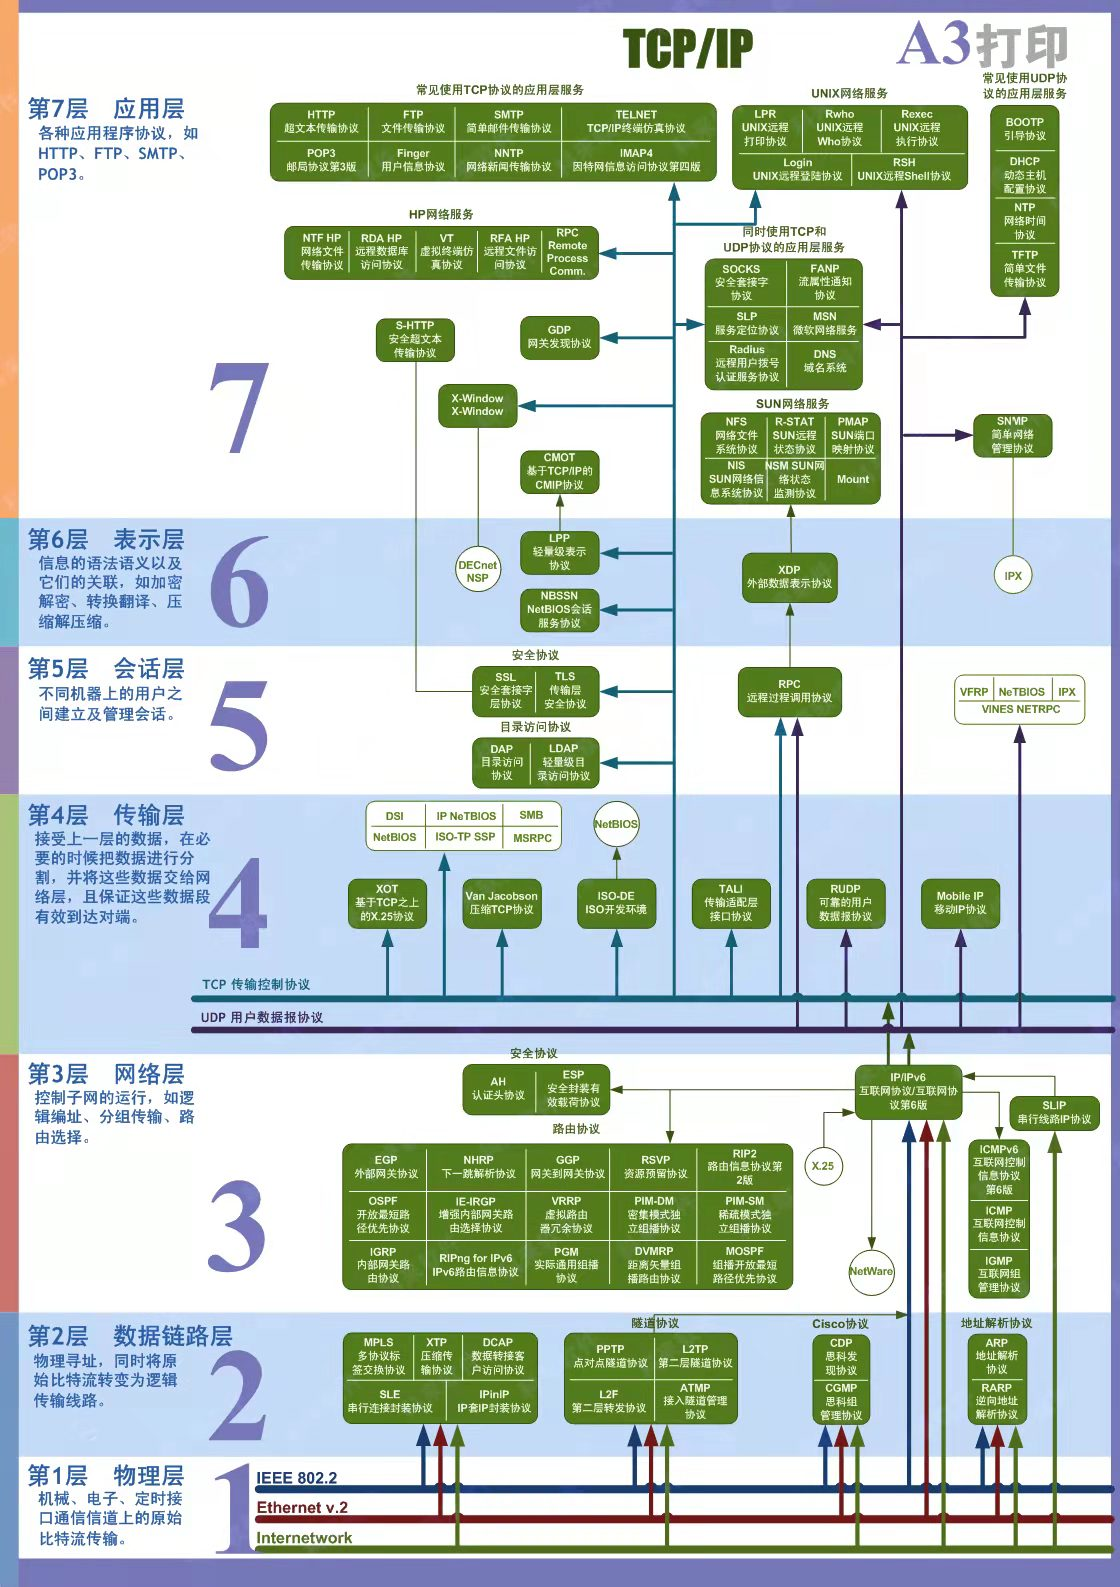
\includegraphics[width=1.3\textwidth]{Fina.jpg}
    \label{fig::100}
\end{figure} 

\end{document}%文章结束